\section{倒立振子のモデリング}
実験目的を達成する制御システムを設計するためにまず、倒立振子系について、状態方程式と観測方程式から成る数式モデルを導出する。
\subsection{状態方程式}
	\begin{figure}[H]
		\centering
		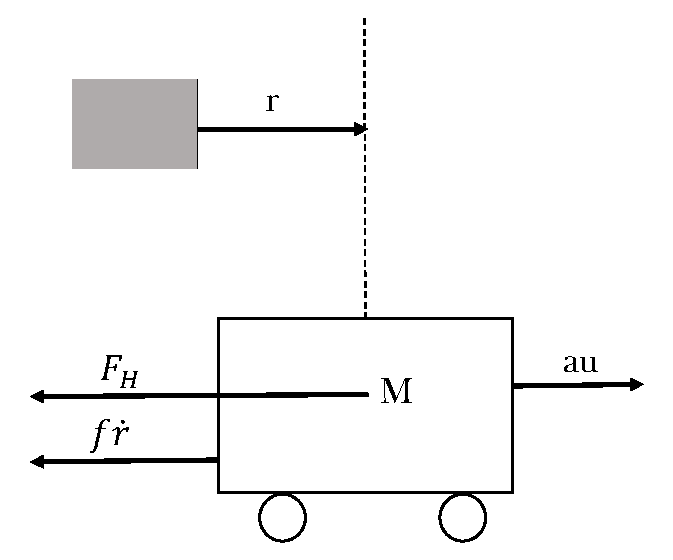
\includegraphics[width=0.4\linewidth]{gazo/cart.eps}
		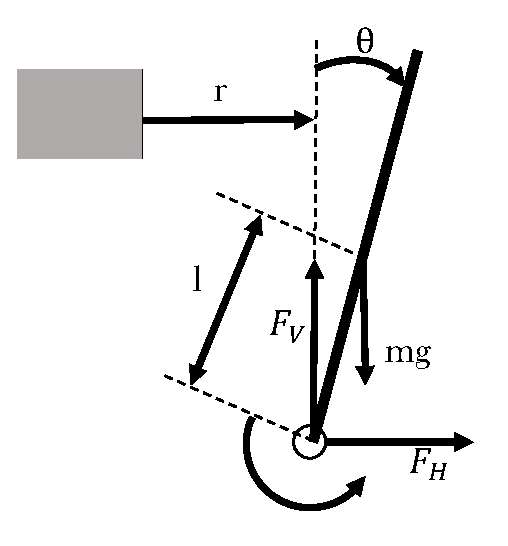
\includegraphics[width=0.4\linewidth]{gazo/stick.eps}
		\caption{数式モデル導出のための参考図}
		\label{image:reference}
	\end{figure}	
	図\ref{image:reference}を参考に各運動方程式を導出すると、\\
	台車の運動方程式は\\
	
	\begin{equation}
		M\ddot{r}=au-F_{H}-f\dot{r}
		\label{eq:motion_eq_cart}
	\end{equation}
	
	倒立振子の回転の運動方程式は
	
	\begin{equation}
		J\ddot{\theta}=lF_{V}\sin \theta -lF_{H}\cos \theta -c\dot{\theta}
		\label{eq:rotemotion_eq_stick}
	\end{equation}
	\\
	倒立振子の水平方向の運動方程式は
	
	\begin{equation}
		m\frac{d^{2}}{dt^{2}}(r+l\sin\theta) = F_{H}
		\label{eq:horizonmotion_eq_stick}
	\end{equation}
	倒立振子の垂直方向の運動方程式は
	
	\begin{equation}
		m\frac{d^{2}}{dt^{2}}(l\cos\theta) = F_{V}-mg
		\label{eq:vertical_eq_stick}
	\end{equation}
	
	となる。
	\par
	ここで各式の導出過程を述べる。図\ref{image:reference}より台車の運動方程式は、振り子からの水平抗力$F_{H}$を考慮してニュートンの第二法則より(\ref{eq:motion_eq_cart})
	式を導くことができる。
	ただし、$M$は台車の質量、$f$は台車の摩擦係数、$a$は駆動アンプへの入力電圧から台車への駆動までのゲイン、$u$はモータの駆動アンプへの入力電圧、$r$は台車の基準位置からの変位である。
	同様にニュートンの第二法則を用いることでそれぞれの方向における(\ref{eq:horizonmotion_eq_stick}),(\ref{eq:vertical_eq_stick})式の運動方程式を導くことができる。
	ただし、$m$は振り子の質量、$l$は回転軸・重心間の距離、$g$は重力加速度、$F_{V}$は振り子が台車から受ける垂直抗力である。
	また、$\theta$は鉛直上向きを$\theta=0$としたときの角度である。
	\par
	最後に(\ref{eq:rotemotion_eq_stick})式は回転に対する運動方程式を考えることで上記と同様に求めることができる。
	ただし、$J$は重心回りの慣性モーメント、$c$は回転軸摩擦係数である。
	\par
	いま、4つの状態変数から成るベクトル、すなわち状態$x$を
					
	\[
		x=\left[
		\begin{array}{ccc}
			r\\
			\theta\\
			\dot{r}\\
			\dot{\theta}\\
		\end{array}
		\right]
		\label{eq:array1}
	\]
					
	のように定義し、(\ref{eq:motion_eq_cart})式,(\ref{eq:rotemotion_eq_stick})式,(\ref{eq:horizonmotion_eq_stick})式,(\ref{eq:vertical_eq_stick})式
	から倒立振子系の非線形状態方程式を求める。
	
	\begin{eqnarray}
		\dot{x} = f(x,u) = \left[
		\begin{array}{ccc}
			\dot{r}\\
			\dot{\theta}\\
			\ddot{r}\\
			\ddot{\theta}\\
		\end{array}
		\right]
		\label{eq:array2}
	\end{eqnarray}
					
	ここで(\ref{eq:horizonmotion_eq_stick})式より$F_{H}$を、
	(\ref{eq:vertical_eq_stick})式より$F_{V}$を求めると
	
	\begin{align}
		F_{H} &= m\frac{d^{2}}{dt^{2}}r + ml\frac{d^{2}}{dt^{2}}\sin{\theta} \notag \\
		&= m\ddot{r}+ml(-\dot{\theta}^{2}\sin{\theta}+\ddot{\theta}\cos{\theta})
		\label{eq:eq1}
	\end{align}
	
	\begin{align}
		F_{V} &= mg + m\frac{d^{2}}{dt^{2}}(l\cos{\theta}) \notag \\
		&= mg + ml(-\dot{\theta}^{2}\cos{\theta}-\ddot{\theta}\sin{\theta})
		\label{eq:eq2}
	\end{align}
	
	である。\\
	(\ref{eq:eq1})式を(\ref{eq:motion_eq_cart})式に代入すると
	
	\begin{equation}
		(M+m)\ddot{r} + ml\ddot{\theta}\cos{\theta}-ml\dot{\theta}^{2}\sin{\theta}+f\dot{r}=au
		\label{eq:eq3}
	\end{equation}
	
	である。\\
	(\ref{eq:eq1})式と(\ref{eq:eq2})式を(\ref{eq:rotemotion_eq_stick})式に代入すると
	
	\begin{equation}
		(J + ml^{2})\ddot{\theta} + ml\ddot{r}\cos{\theta} - mgl\sin{\theta} + c\dot{\theta} = 0
		\label{eq:eq4}
	\end{equation}
	
	である。\\
	(\ref{eq:eq3})式、(\ref{eq:eq4})式を行列表現すると
	
	\[
		\left[
		\begin{array}{ccc}
			(M + m)\ddot{r} + (ml\cos{\theta})\ddot{\theta} + (-ml\sin{\theta}) + f\dot{r} = au \\
			(ml\cos{\theta})\ddot{r} + (J + ml^{2})\ddot{\theta} -mgl\sin{\theta} + c\dot{\theta} = 0\\
		\end{array}
		\right]
	\]
	
	\[
		\left[
		\begin{array}{ccc}
			M + m & ml\cos{\theta} \\
			ml\cos{\theta} & J + ml^{2}\\
		\end{array}
		\right]
		\left[
		\begin{array}{ccc}
			\ddot{r} \\
			\ddot{\theta}\\
		\end{array}
		\right] +
		\left[
		\begin{array}{ccc}
			-ml\ddot{\theta}^{2}\sin{\theta} + f\dot{r}\\
			mgl\sin{\theta} + c\dot{\theta}\\
		\end{array}
		\right] = 
		\left[
		\begin{array}{ccc}
			au\\
			0\\
		\end{array}
		\right]
	\]
	
	$\begin{pmatrix} M + m & ml\cos{\theta} \\ ml\cos{\theta} & J + ml^{2} \end{pmatrix}$を$K$と置いて右辺に逆行列としてかけると\\
	
	\[
		\left[
		\begin{array}{ccc}
			\ddot{r}\\
			\ddot{\theta}\\
		\end{array}
		\right]=K^{-1}
		\left[
		\begin{array}{ccc}
			au-f\dot{r}+ml\ddot{\theta}\sin{\theta}\\
			mgl\sin{\theta} - c\dot{\theta}\\
		\end{array}
		\right]
	\]
	\\
	よって以上から(\ref{eq:array2})式は\\
	
	\begin{equation}
		\dot{x} = f(x,u)=\left[
		\begin{array}{ccc}
			\dot{r}\\
			\dot{\theta}\\
			K^{-1}\left[
			\begin{array}{ccc}
				-f\dot{r}+ml\ddot{\theta}\sin{\theta}+au\\
				mgl\sin{\theta}-c\dot{\theta}
			\end{array}
			\right]
		\end{array}
		\right]
		\label{eq:array3}
	\end{equation}
	\\
	となる。ただし、$K$は
	
	\begin{equation}
		K=\left[
		\begin{array}{ccc}
			M+m & ml\cos{\theta}\\
			ml\cos{\theta} & J+ml^{2}\\
		\end{array}
		\right]
		\label{eq:array4}
	\end{equation}
	
	である。
	よって倒立振子系の非線形状態方程式は(\ref{eq:array3})式のように得られる。
	\par
	ところで、倒立振子系については、その制御目的から、不安定平衡点$x=0$の近傍での挙動を表す
	状態方程式を知れば十分である。そこで、この基準状態まわりで一時近似された状態方程式を求め
	ることを考える。\\
	(\ref{eq:array3})式に一次近似のテイラー展開を施すと、\\
	\begin{equation}
		f(x,u) = f(0,0) + \left.\frac{\partial f}{\partial x}\right|_{x=0,u=0}(x-0) + \left.\frac{\partial f}{\partial u}\right|_{x=0,u=0}(u-0)
		\label{eq:eq4}
	\end{equation}
	\\
	となる。つまり、(\ref{eq:eq4})を計算すれば求めたい状態方程式を得ることができる。\\
	(\ref{eq:eq4})式において、
	
	\[A=\left.\frac{\partial f}{\partial x}\right|_{x=0,u=0} , B=\left.\frac{\partial f}{\partial u}\right|_{x=0,u=0}\]
	
	とすると、(\ref{eq:eq4})式は以下のように計算できる。
	\begin{equation}
		f(x,u) = Ax+Bu
		\label{eq:AxBu}
	\end{equation}
	ここで、一時近似を施したので、$\theta$を微小範囲と考えることができ、\\ $\sin{\theta} \simeq  \theta , \cos{\theta} \simeq 1 , \dot{\theta}^{2} \simeq 0$のように
	近似できる。\\
	以上の近似から(\ref{eq:array3}),(\ref{eq:array4})式は\\
	\begin{equation}
		f(x,u)=\left[
		\begin{array}{ccc}
			\dot{r}\\
			\dot{\theta}\\
			K^{'-1}\left[
			\begin{array}{ccc}
				au-f\dot{r}\\
				mlg\theta-c\dot{\theta}\\
			\end{array}
			\right]
		\end{array}
		\right]
		\label{eq:array5}
	\end{equation}
	
	\begin{equation}
		K^{'} = \left[
		\begin{array}{ccc}
			M + m & ml\\
			ml & J+ml^{2}\\
		\end{array}
		\right]
		\label{eq:array6}
	\end{equation}
	
	となる。ここで、(\ref{eq:array5})式の3行目を$a_{1}$と置き、4行目を$a_{2}$と置く。\\\newpage
	(\ref{eq:array5})、(\ref{eq:array6})式を用いて(\ref{eq:AxBu})式のA、Bを計算する。\\
	
	\begin{align*}
		A=\frac{\partial \textgt{f}}{\partial \textgt{x}}&=
		\left[
		\begin{array}{cccc}
			\frac{\partial \dot{r}}{\partial r} & \frac{\partial \dot{r}}{\partial \theta} & \frac{\partial \dot{r}}{\partial \dot{r}} & \frac{\partial \dot{r}}{\partial \dot{\theta}} \\
			\frac{\partial \dot{\theta}}{\partial r} & \frac{\partial \dot{\theta}}{\partial \theta} & \frac{\partial \dot{\theta}}{\partial \dot{r}} & \frac{\partial \dot{\theta}}{\partial \dot{\theta}} \\
			\frac{\partial a_{1}}{\partial r} & \frac{\partial a_{1}}{\partial \theta} & \frac{\partial a_{1}}{\partial \dot{r}} & \frac{\partial a_{1}}{\partial \dot{\theta}} \\
			\frac{\partial a_{2}}{\partial r} & \frac{\partial a_{2}}{\partial \theta} & \frac{\partial a_{2}}{\partial \dot{r}} & \frac{\partial a_{2}}{\partial \dot{\theta}} \\
		\end{array} 
		\right]  \\
		&=\left[
		\begin{array}{cccc}
			0 & 0 & 1 & 0 \\
			0 & 0 & 0 & 1 \\
			0 & 0 & K^{'-1}(-f) & 0\\
			0 & K^{'-1}(mgl) & 0 & K^{'-1}(-c) \\
		\end{array}
		\right]
	\end{align*}
	\\
	\[
		B=\frac{\partial \textgt{f}}{\partial \textgt{u}}=
		\left[
		\begin{array}{c}
			\frac{\partial \dot{r}}{\partial u}\\
			\frac{\partial \dot{\theta}}{\partial u}\\
			\frac{\partial a_{1}}{\partial u}\\
			\frac{\partial a_{2}}{\partial u}\\
		\end{array}
		\right]=
		\left[
		\begin{array}{c}
			0\\
			0\\
			K^{'-1}a\\
			0\\
		\end{array}
		\right]
		\label{eq:array7}
	\]
	\\
	以上から線形状態方程式は\\
	\[\dot{x}=A\textgt{x}+B\textgt{u}\]
	\begin{equation}
		=\left[
		\begin{array}{cccc}
			0 & 0 & 1 & 0 \\
			0 & 0 & 0 & 1 \\
			0 & 0 & K^{'-1}(-f) & 0 \\
			0 & K^{'-1}(mgl) & 0 & K^{'-1}(-c)\\
		\end{array}
		\right]
		\left[
		\begin{array}{c}
			r\\
			\theta\\
			\dot{r}\\
			\dot{\theta}\\
		\end{array}
		\right] + 
		\left[
		\begin{array}{c}
			0\\
			0\\
			K^{'-1}au\\
			0\\
		\end{array}
		\right]
		\label{eq:InPeAboveLiner}
	\end{equation}
	\\
	となる。ただし、$K^{'}$は(\ref{eq:array6})式である。上式の線形状態方程式は鉛直上向きを$\theta = 0$としたときの状態方程式である。
	鉛直下向きを$\theta = 0$とした場合は(\ref{eq:array4})式の三角関数内の
	$\theta$に+$\pi$すればよいので
	\begin{equation}
		\dot{x} = f(x,u)=\left[
		\begin{array}{ccc}
			\dot{r}\\
			\dot{\theta}\\
			K^{-1}\left[
			\begin{array}{ccc}
				-f\dot{r}-ml\ddot{\theta}\sin{\theta}+au\\
				-mgl\sin{\theta}-c\dot{\theta}
			\end{array}
			\right]
		\end{array}
		\right]
		\label{eq:InPeUnderNonLiner}
	\end{equation}
	\\
	となる。ただし、$K$は
	\begin{equation}
		K=\left[
		\begin{array}{ccc}
			M+m & -ml\cos{\theta}\\
			-ml\cos{\theta} & J+ml^{2}\\
		\end{array}
		\right]
		\label{eq:InPeUnderNonLinerK}
	\end{equation}
	である。\\
	振子の角度を鉛直上向きを$\theta=0$としたときの状態方程式を線形化したときと同様に
	(\ref{eq:InPeUnderNonLiner}),(\ref{eq:InPeUnderNonLinerK})式を線形化すると
	線形状態方程式は\\
	\[\dot{x}=A\textgt{x}+B\textgt{u}\]
	\begin{equation}
		=\left[
		\begin{array}{cccc}
			0 & 0 & 1 & 0 \\
			0 & 0 & 0 & 1 \\
			0 & 0 & K^{'-1}(-f) & 0 \\
			0 & K^{'-1}(-mgl) & 0 & K^{'-1}(-c)\\
		\end{array}
		\right]
		\left[
		\begin{array}{c}
			r\\
			\theta\\
			\dot{r}\\
			\dot{\theta}\\
		\end{array}
		\right] + 
		\left[
		\begin{array}{c}
			0\\
			0\\
			K^{'-1}au\\
			0\\
		\end{array}
		\right]
		\label{eq:InPeUnderLiner}
	\end{equation}
	\\
	となる。ただし、$K$は、
	\[
		K=\left[
		\begin{array}{ccc}
			M+m & -ml\\
			-ml & J+ml^{2}\\
		\end{array}
		\right]
	\]
	である。\\
	今後、(\ref{eq:InPeAboveLiner})式を鉛直上向き基準の線形状態方程式とし、
	(\ref{eq:InPeUnderLiner})式を鉛直下向き基準の線形状態方程式とする。
	
\subsection{観測方程式}
	2つの観測出力は
	\[
		y_{1} = c_{1}r\\
	\]
	\[
		y_{2} = c_{2}\theta\\
	\]
	のように表される。ここで、$c_{1}$は変位・電圧変換係数、$c_{2}$は角度・電圧変換係数である。これから成るベクトル出
	力$y$を\\
	\[
		y=\left[
		\begin{array}{c}
			y_{1}\\
			y_{2}\\
		\end{array}
		\right]
	\]
	のように定義すると、倒立振子系に対する観測方程式として\\
	\begin{align}
		y&=Cx \notag \\
		\left[
		\begin{array}{c}
			y_{1}\\
			y_{2}\\
		\end{array}
		\right]&=\left[
		\begin{array}{cccc}
			c_{1} & 0 & 0 & 0 \\
			0 & c_{2} & 0 & 0\\
		\end{array}
		\right]\left[
		\begin{array}{c}
			r\\
			\theta\\
			\dot{r}\\
			\dot{\theta}\\
		\end{array}
		\right]
		\label{eq:output}
	\end{align}
	を得ることができる。\\
	なお、鉛直上向きを基準とした場合でも鉛直下向きを基準とした場合でも出力方程式は変わらない。
%一次チェック完了:
%----------------------------------------------------------------------------------------------------
\section{倒立振子のパラメータの同定}
数式モデル(\ref{eq:array6})、(\ref{eq:array7})、(\ref{eq:output})に含まれる物理パラメータを実際の倒立振子系で実験
を行い同定する。
\subsection{mとlの測定}
	倒立振子系から振子を取り外し、バネ秤で振子の質量$m$を測定する。つぎに、振子を鋼尺のエッジ上でバランス
	させて、重心の位置を定め、$l$を測定する。
	以下に測定した結果を示す。
	\[m = 0.031[\rm{kg}]\]
	\[l = 0.15[\rm{m}]\]
\subsection{aの測定}
	モータに一定電圧を加え、ばねばかりで台車を引き、台車が正の方向に動き出すときの力($au+摩擦力$)を$f_{max}$
	、負の方向に動き出すときの力($au-摩擦力$)を$f_{min}$とする。図\ref{image:parameterA}に示すように
	$u$と$f_{max},f_{min}$の関係をいくつかの電圧について調べ、最小2乗法によって1次関数を求め、この傾きを
	$a$とする。\cite{Koga:Binpe}
	\begin{figure}[H]
		\centering
		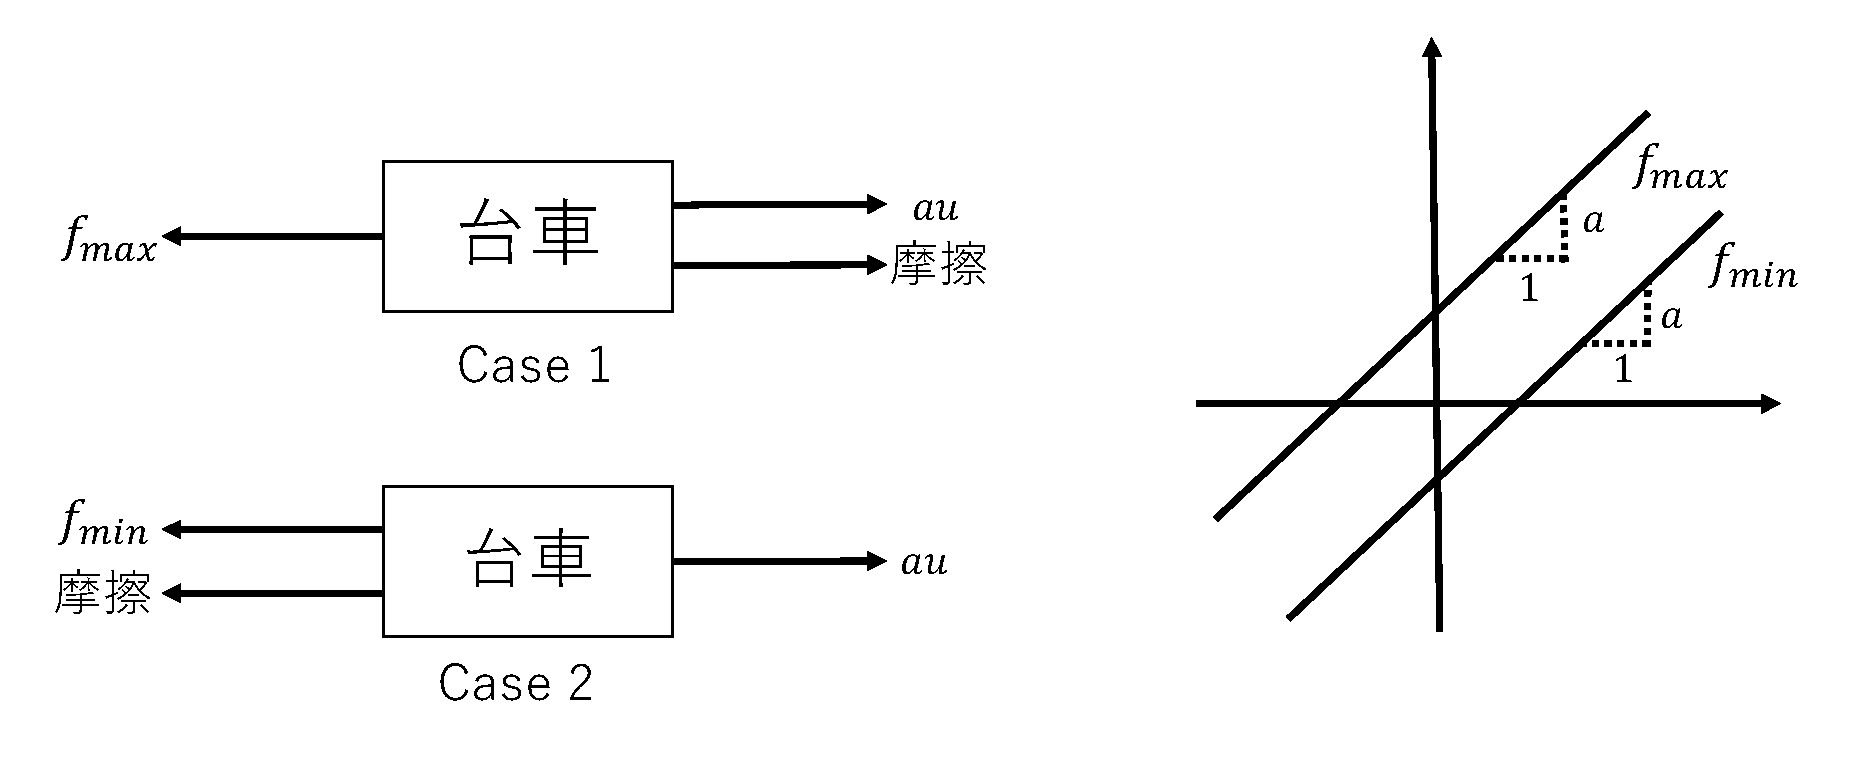
\includegraphics[width=1.0\linewidth]{gazo/ParameterA.eps}
		\caption{パラメータaの決定}
		\label{image:parameterA}
	\end{figure}
	なお、振子は台車から取り外して測定を行う。
	以下に測定した結果から得られた一次関数の傾き$a$を示す。
	\[
		a=0.062[\rm{Kg/V}] = 0.61[\rm{N/V}]
	\]
	
\subsection{Jとcの測定}
	振子を自由振動させることにより、$J$と$c$を測定できる。その数式モデルは鉛直下向きを基準として
	\begin{equation}
		(J + ml^{2})\ddot{\theta} - mgl\sin{\theta} + c\dot{\theta} = 0
		\label{eq:Para1}
	\end{equation}
	\begin{equation}
		y_{2} = c_{2}\theta
	\label{eq:Para2}
	\end{equation}
	で与えられる。$\theta$を微小範囲で考えると、(\ref{eq:Para1}),(\ref{eq:Para2})式は
	\[
		\ddot{y}_{2} + 2\zeta\omega_{n}\dot{y}_{2} + \omega_{n}^{2}y_{2} = 0
	\]
	ただし、
	\[
		\zeta = \frac{c}{2\sqrt{mgl\left(J + ml^{2}\right)}} 
		,\ \  \omega_{n} = \sqrt{\frac{mgl}{J+ml^{2}}}
	\]
	のように書くことができる。この解は
	\[0<\zeta<1\]
	のとき、減衰振動となり
	\[
		y_{2}(t) = \frac{y_{2}(0)}{\sqrt{1-\zeta^{2}}}\exp{(-\omega_{n}\zeta t)}
	  	\sin{(\omega_{n}\sqrt{1-\zeta^{2}}t + \phi)}
	\]
	ただし
	\[
		\phi = \tan^{-1}{\frac{\sqrt{1-\zeta^2}}{\zeta}}
	\]
	で与えられる。\cite{Koga:Binpe}
	\begin{figure}[H]
		\centering
		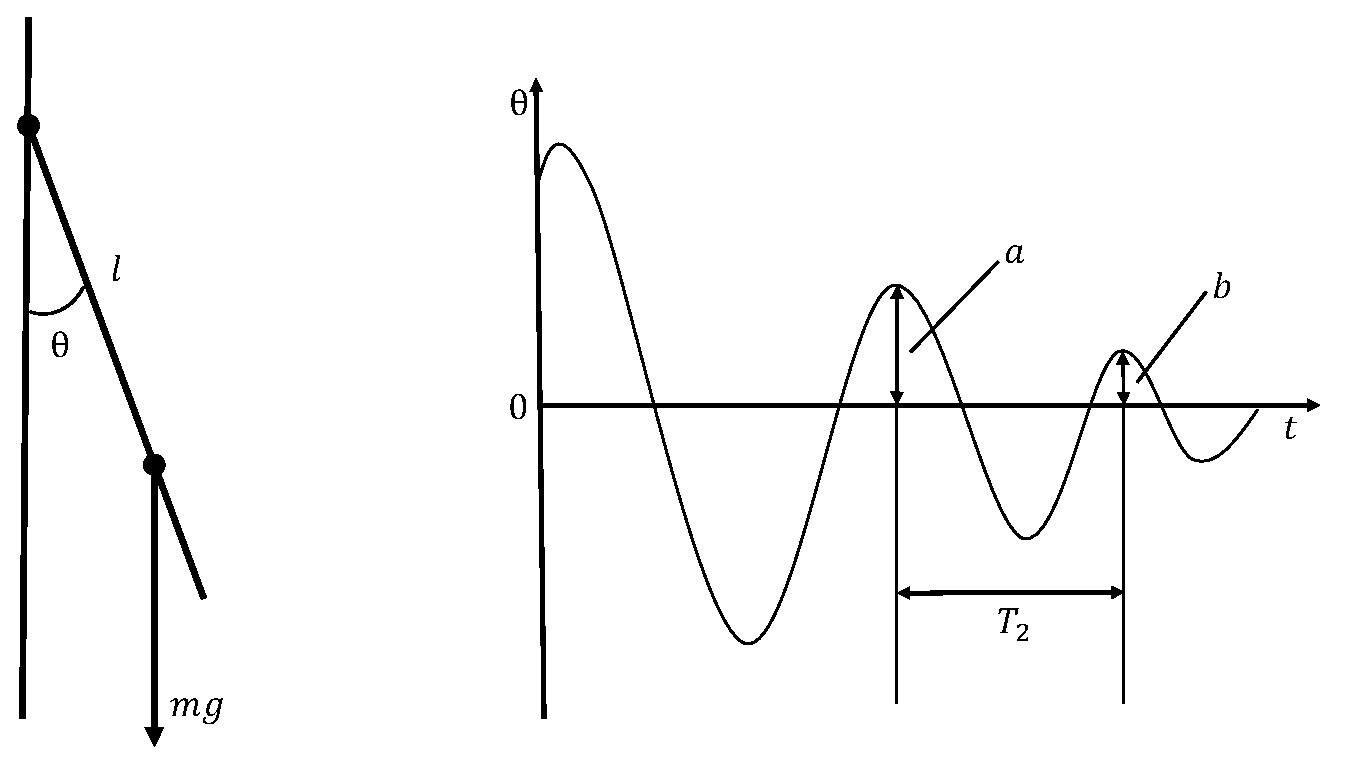
\includegraphics[width=1.0\linewidth]{gazo/ParameterJC.eps}
		\caption{$J$と$c$の測定}
		\label{image:parameterJC}
	\end{figure}
	\par
	いま、減衰振動の周期を$T_{2}$とし、時刻$t_{1}$と時刻$t_{2} = t_{1}+T_{2}$において波形
	$y_{2}(t)$の山が隣合うものとする。このときの振幅の減衰比は
	\[
		\frac{|y_{2}(t_{2})|}{|y_{2}(t_{1})|} = \exp{(-\lambda)}
	\]
	ただし
	\[
		\lambda = \frac{2\pi\zeta}{\omega_{n}\sqrt{1-\zeta^2}} 
	\]
	となる。この$\lambda$は対数減衰比と呼ばれる。また
	\[
		T_{2} = \frac{2\pi}{\omega_{n}\sqrt{1-\zeta^{2}}}
	\]
	が成り立つ。したがって、$J$と$c$は
	\[
		J=\frac{mglT_{2}^{2}}{4\pi^{2}+\lambda^{2}}-ml^{2},\ \ 
		c=\frac{2\lambda(J+ml^{2})}{T_{2}}
	\]
	のように与えられる。\cite{Koga:Binpe}
	以下に振子を自由振動させ得られたデータから計算した$J$と$c$を示す。
	\[
		J=2.5\times10^{-4}[\rm{khm^{2}}]
	\]
	\[
		c=5.4\times10^{-5}[\rm{kgm^{2}/s}]
	\]
	
\subsection{Mとfの測定}
	
	$M$と$f$の測定方法には二通りがある。
	\subsubsection{ステップ応答による測定法}
		ここでは、台車をアンプ・モータプーリ・ベルト・台車系の等価質量と等価摩擦係数とし、
		台車のステップ応答を測定することで$M$と$f$を決定する。
		ただし、振り子は台車から取り外した状態で測定を行う。
		このときの運動方程式は
		\[
			M\ddot{r} = au - f\dot{r}
		\]
		であり、$u$から$r$までの伝達関数$G$は
		\[
			G(s) = \frac{K}{s(Ts+1)}
		\]
		となる。ただし、
		\begin{equation}
			K = \frac{a}{f},\ \ T=\frac{M}{f}
			\label{eq:kt}
		\end{equation}
		である。初期状態を0とするとき、このシステムのステップ応答は
		\begin{equation}
			r(t) = KU_{0}\left(Te^{\frac{-t}{T}}+t-T\right)
			\label{eq:step}
		\end{equation}
		である。
		\begin{figure}[H]
			\centering
			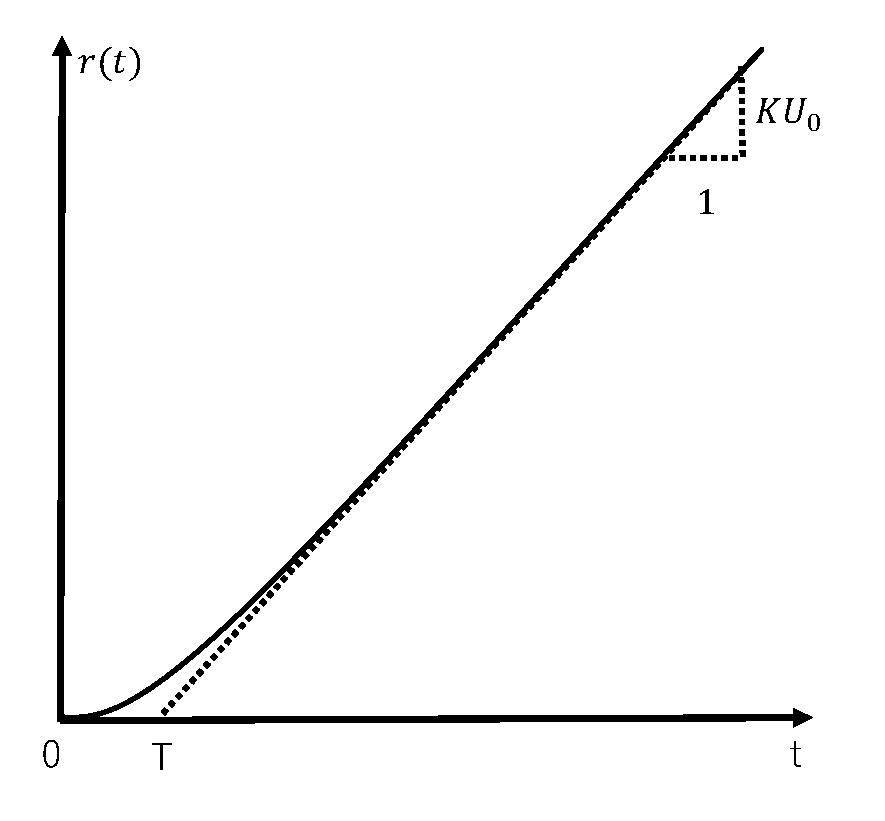
\includegraphics[width=0.6\linewidth]{gazo/step.eps}
			\caption{台車のステップ応答}
			\label{image:parameterMF}
		\end{figure}
		ただし、$U_{0}$はステップの高さである。
		(\ref{eq:step})において$t→\infty$とすれば
		\[
			r(t) = KU_{0}(t-T)
		\]
		となり、図\ref{image:parameterMF}を参考に$T$と$K$をもとめ、
		(\ref{eq:kt})式より$M$と$f$を決定することができる。
		以下にこの方法を用いて同定したパラメータを示す。
		\[
			M=6.9E-1[\rm{kg}]
		\]
		\[
			f=7.6[\rm{kg/s}]
		\]
		
	\subsubsection{フィードバック入力による測定法}
		ここでは、入力にステップ応答ではなく、以下に示すようなフィードバック入力を加える。
		\begin{equation}
			u = k_{c}(y_{c} - y)
		\end{equation}
		ただし、$y_c$は目標値、$y$は出力、$k_{c}$はフィードバックゲインである。
		本節では$k_c=2500$とする。
		このようにすることで不足制動の2次系($\zeta<1$)を実現させる。
		\begin{figure}[H]
			\centering
			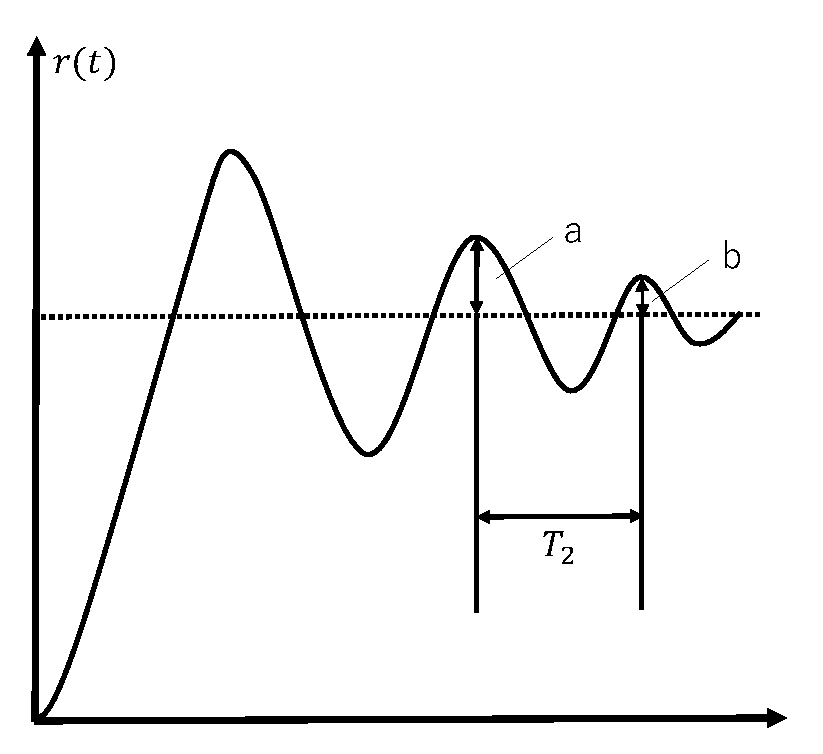
\includegraphics[width=0.6\linewidth]{gazo/feedback.eps}
			\caption{台車のフィードバック応答}
			\label{image:parameterMFfeed}
		\end{figure}
		図\ref{image:parameterMFfeed}を参考にして$M$と$f$を同定する。
		この方法は$J$と$c$の同定の際に用いた方法とほぼ同じであるため、詳しい説明はそちらに
		譲る。
		\par
		台車のフィードバック応答から求めた$\lambda$と$T_2$から以下の式を用いて$\zeta$と$\omega_{n}$を計算し求める。
		\begin{equation}
			\lambda=\frac{2\pi\zeta}{\sqrt{1-\zeta^{2}}}
		\end{equation}
		\begin{equation}
			T_{2}=\frac{2\pi}{\omega_{n}\sqrt{1-\zeta^{2}}}
		\end{equation}
		上の式を式変形して$\zeta$と$\omega_{n}$イコールの式にすると
		\begin{equation}
			\zeta=\frac{\lambda}{\sqrt{4\pi^{2}+\lambda^{2}}}
		\end{equation}
		\begin{equation}
			\omega_{n}=\frac{2\pi}{T_{2}\sqrt{1-\zeta^{2}}}
		\end{equation}
		以上の式から求めた$\zeta$と$\omega_{n}$は以下の二次系の伝達関数の基本形に代入することで
		同定に用いたフィードバック制御系の伝達関数を求めることができる
		\begin{equation}
			G(s) = \frac{\omega_{n}^{2}}{s^{2}+2\zeta\omega_{n}s + \omega_{n}^{2}}
		\end{equation}
		また、今回のフィードバック制御系におけるブロック線図は以下のようになる。
		\begin{figure}[H]
			\centering
			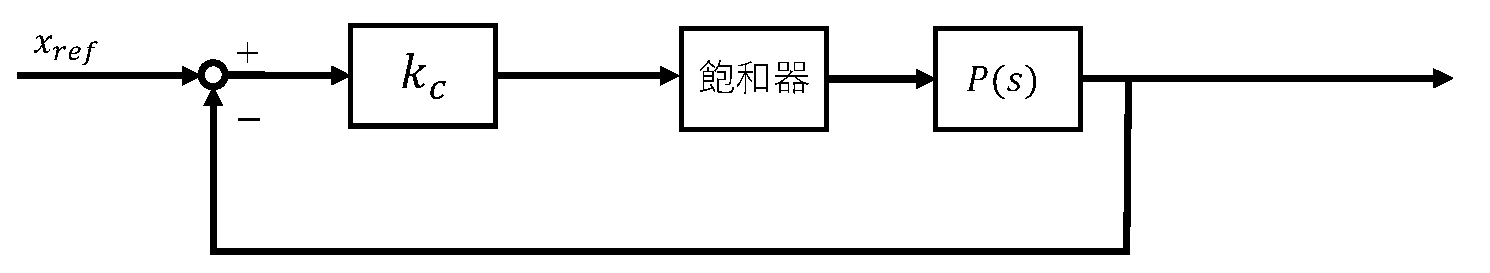
\includegraphics[width=1.0\linewidth]{gazo/FeedBackCart.eps}\\
			\caption{フィードバック制御系のブロック線図}
			\label{image:FeedBackCart}
		\end{figure}
		ここで、$P(s)$は台車の伝達関数であり以下の式で表される。
		\begin{equation}
			P(s)=\frac{K}{s(Ts+1)}
			\label{eq:Ps}
		\end{equation}
		ただし、Tは$M/f$、Kは$a/f$である。上のブロック線図から伝達関数を求める。
		しかし、飽和システムを含んでいると伝達関数を求めることができないので、ここでは飽和システムがなくても
		台車は問題なく動作するものとして仮定する。以上の仮定から伝達関数は
		\begin{equation}
			G(s) = \frac{AK/T}{s^{2}+(1/T)s+(AK/T)}
			\label{eq:Gs}
		\end{equation}
		となる。ただしAはゲインである。(\ref{eq:Ps})式と(\ref{eq:Gs})式を係数比較し、$M,f$イコール
		の式にすると以下のようになる。
		\begin{equation}
			\left.
			\begin{array}{l}
				\displaystyle M=\frac{aA}{\omega_{n}^{2}} , \ f=2\zeta\omega_{n}^{2}M
			\end{array}
			\right.
			\label{eq:mf}
		\end{equation}
		よって、(\ref{eq:mf})式からMとfは以下のように求まる。
		\[
			M=1.59[\rm{kg}]
		\]
		\[
			f=13.2[\rm{kg/s}]
		\]
		
	\subsubsection{$M$と$f$の決定}
	パラメータ$M$と$f$についてはステップ応答による方法とフィードバックによる方法の2通りから
	同定を行った。しかし、それぞれの方法で求めたパラメータを比較するとまるで違うことがわかる。
	これはフィードバックによる方法が十分に正確な方法ではなかったためといえる。
	その原因は、飽和システムを含めずに同定を行ったことではないかと考える。
	シミュレーションにおいては入力にどのような値を加えても倒立振子系に何ら影響はないが
	実際の倒立振子においてはその入力できる値には制限がある。この制限を考えるか否か
	で結果が変わってくるはずである。
	\begin{figure}[H]
		\centering
		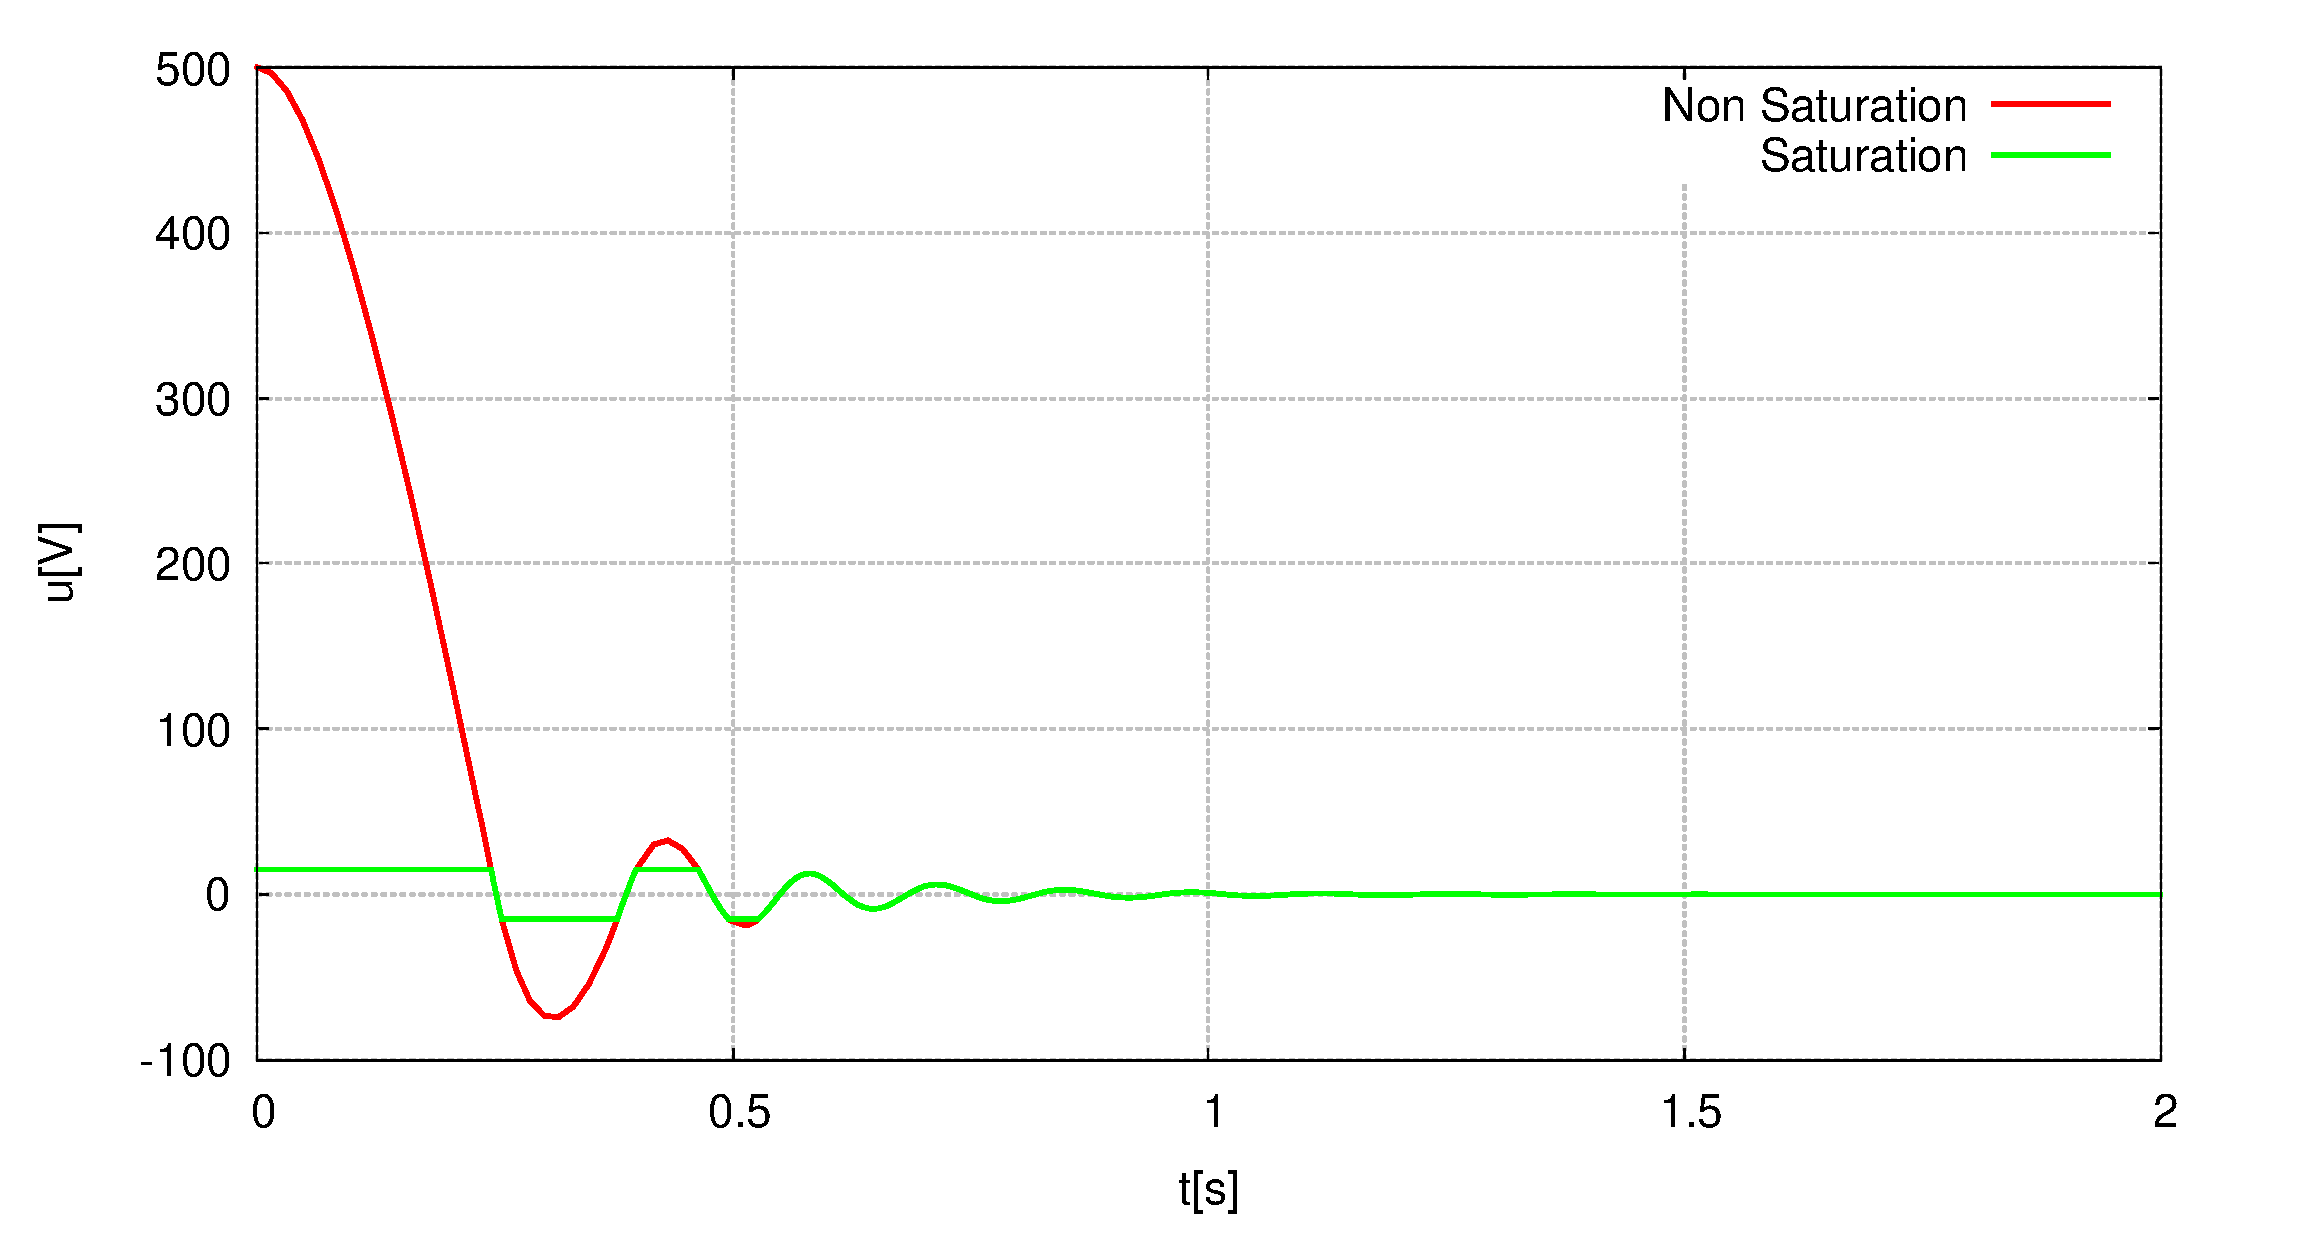
\includegraphics[width=0.8\linewidth]{gazo/feedback_input.eps}\\
		\caption{飽和器の有無によるフィードバック入力の比較}
		\label{image:feedback_saturation}
	\end{figure}
	図\ref{image:feedback_saturation}は図\ref{image:FeedBackCart}のブロック線図において
	飽和器を含めた場合の入力と飽和器を含めなかった場合の入力を描画させたものである。
	この図より、飽和器がない(non Saturation)場合、入力は最大500(V)まで加えられることがわかる。本実験で用いる倒立振子系の入力限界は
	$-15<u<15$であるので、飽和器を加えた場合、その範囲を超える入力は絶対値15(V)に制限されている。
	つまり、フィードバックによる方法で同定したパラメータは飽和器を考慮していないので、現実の倒立振子系とは違うパラメータであるといえる。
	また、今回はフィードバックゲインを2500としたが、
	フィードバックゲインを小さくすると、入力もそれに伴い小さくなるので、
	現実の倒立振子系に近いパラメータを同定することができるはずである。
	以上から本実験においてフィードバックを行う場合、入力が大きく跳ね上がる可能性があるので、必ず飽和システムが必要であるといえる。
	なので、飽和システムが存在する限り伝達関数を求めることができないので、
	正確なパラメータの計算を行うことができないといえる。
	以降、パラメータ$M,f$はステップ応答による方法で同定した値を用いる。
	
\subsection{$c_1$と$c_2$の測定}
	$c_1$と$c_2$に関しては
	\[
		c_1 = 1.0 [\rm{V/m}]
	\]
	\[
		c_2 = 1.0[\rm{V/rad}]
	\]
	というように
	ソフトウェアに設定してあるものを用いた。
\subsection{同定結果}
	同定実験において同定したパラメータを表にまとめる。
	\begin{table}[htb]
		\begin{center}
			\caption{同定したパラメータの一覧}
			\medskip
			
			\begin{tabular}{|l|l|}\hline
				パラメータ & 同定した値 \\ \hline\hline
				m[kg]  & 0.031\\ \hline
				l[m] & 0.15\\ \hline
				M[kg] & 0.69\\ \hline
				f[kg/s] & 7.6\\ \hline
				J[$\rm{kgm}^2$] & $2.5\times10^{-4}$\\ \hline
				c[$\rm{kgm}^2/\rm{s}$] & $5.4\times10^{-5}$\\ \hline
				a[N/V] & 0.61\\ \hline
				$c_{1}$[V/m] & 1.0\\ \hline
				$c_{2}$[V/rad] & 1.0\\ \hline
			\end{tabular}
		\end{center}
	\end{table}
%一次チェック完了:
%-----------------------------------------------------------------------------------------------------	
\section{パラメータの検証}
	前節では、実験によって倒立振子のパラメータを同定した。
	しかし、その同定したパラメータがどれほど有効性があるか現時点では全く分からない状況である。
	そこで、本節では同定したパラメータの有効性をがどれほどなのかシミュレーションを用いて検証を
	行う。シミュレーションに用いたツールはJAMOXである。ただし、直接同定を行った$m,l$や最初から
	設定してあった$c_1,c_2$については検証は行わない。
	\subsection{振子の自由振動シミュレーション}
		ここでは、$J,c$の検証を行う。
		以下にシミュレーションと実験データを描画したグラフを示す。
		\begin{figure}[H]
			\centering
			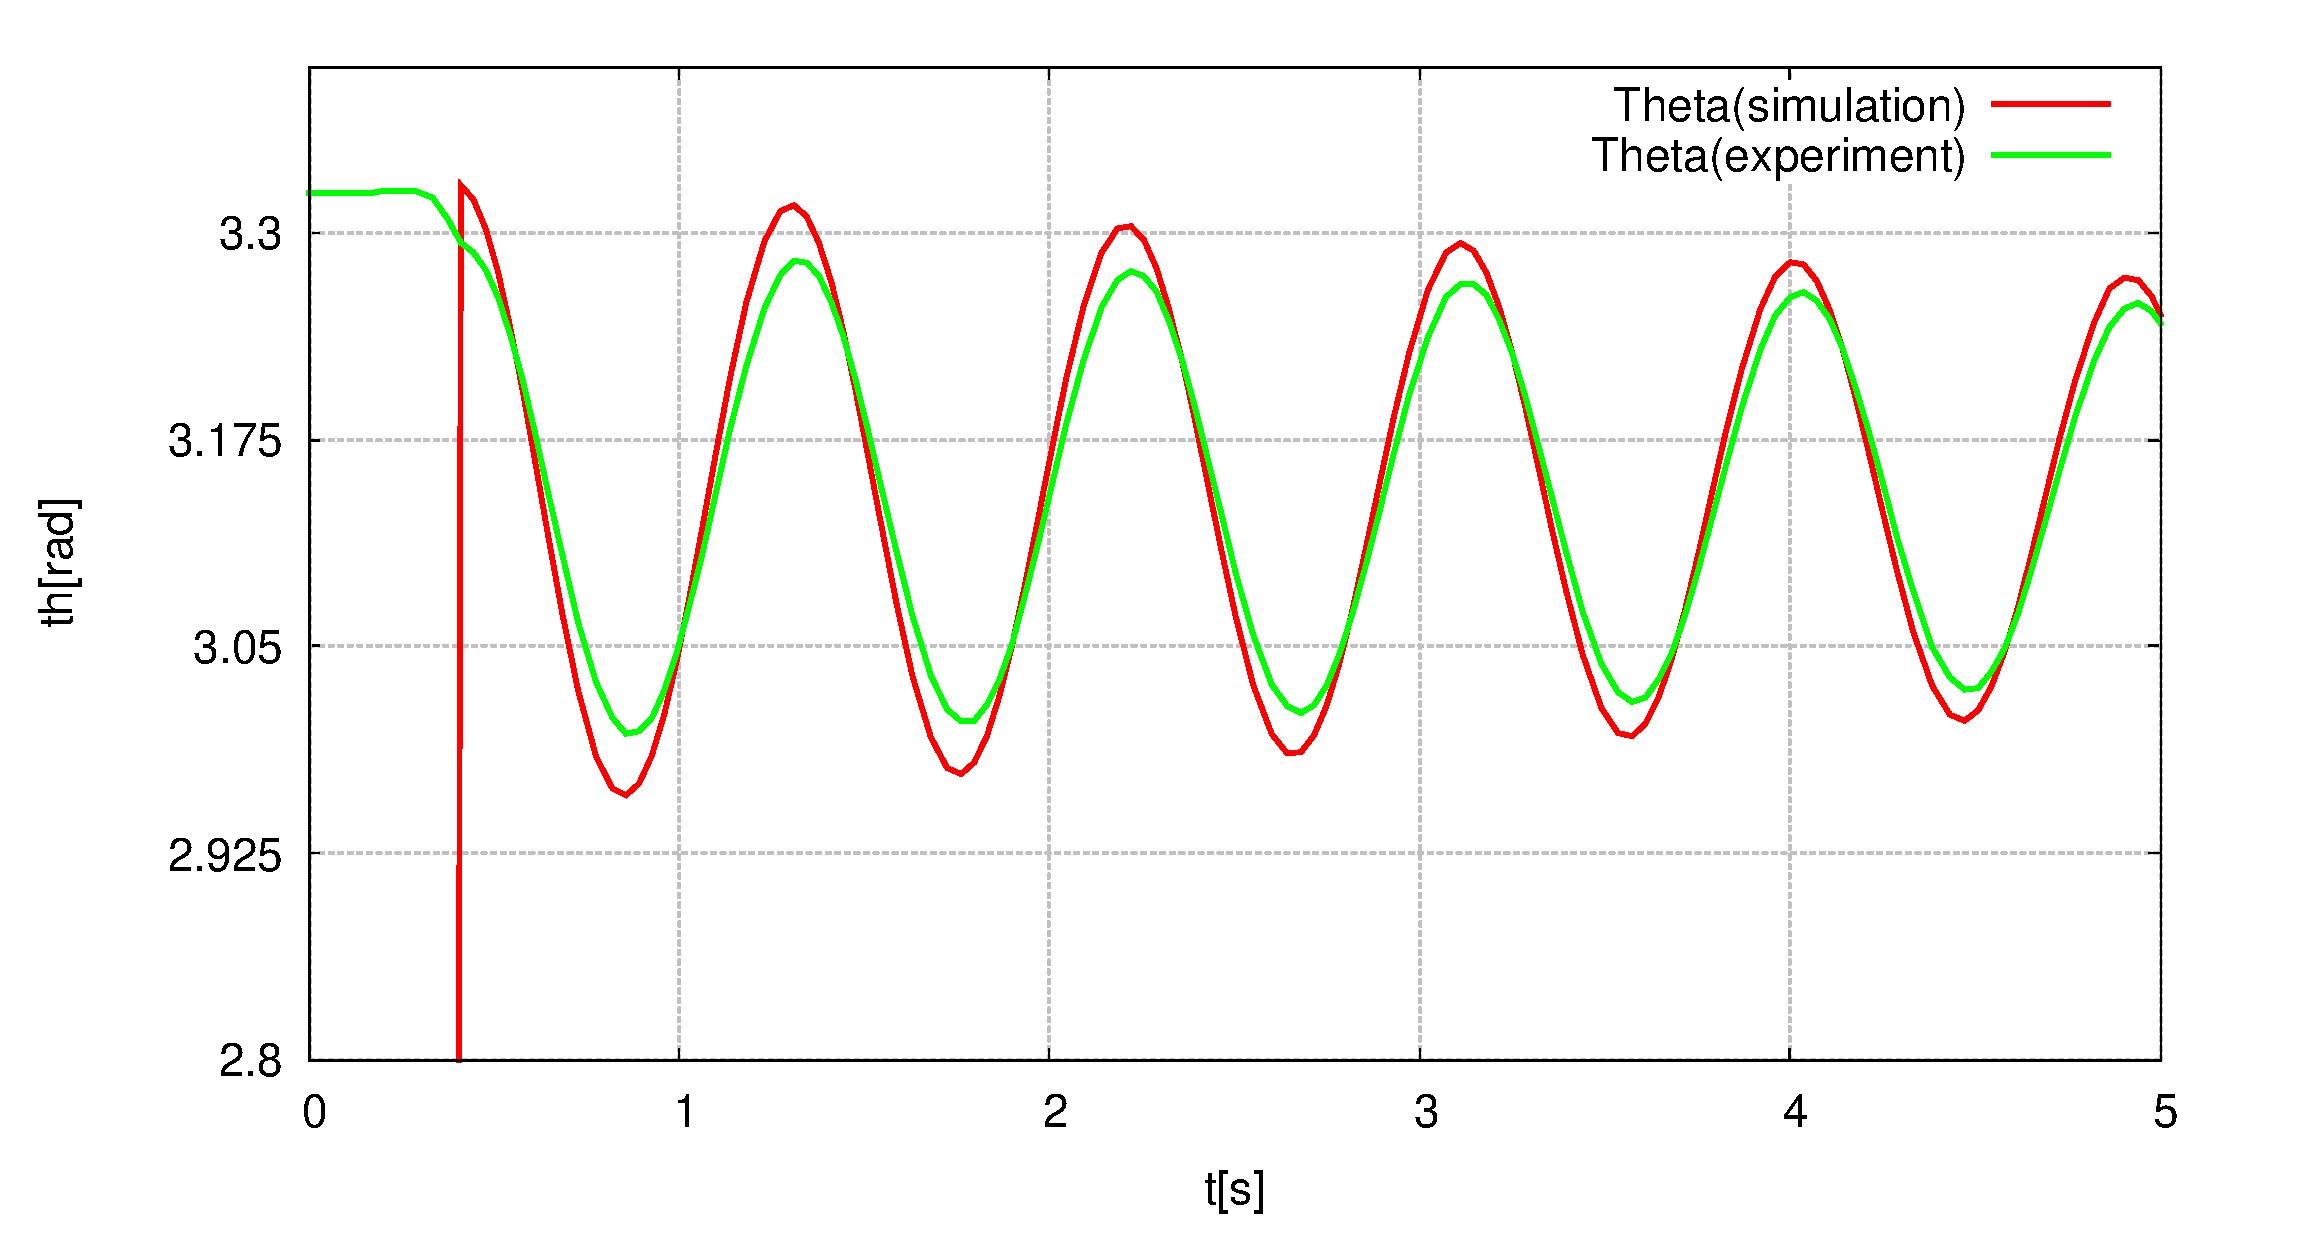
\includegraphics[width=0.8\linewidth]{gazo/free45Auto.eps}\\ 
			\caption{振子の自由振動シミュレーション}
			\label{image:freependulum}
		\end{figure}
		図\ref{image:freependulum}において、シミュレーションは0.32(s)程遅らせて実行しているので、それ以前の時間の角度は$0°$である。
		自由振動の初期角度は$180°$を基準として$10°$である。
		図\ref{image:freependulum}よりシミュレーションと実験結果に少し差異はあるが
		大きな違いはないといえる。よって同定したパラメータ$J,c$は有効な値であるといえる。
		\newpage
	\subsection{台車のステップ応答による方法のシミュレーション}
		ここでは、$M,f,a$の検証を行う。$M,f$はステップ応答による方法で求めた値を用いる。
		以下にシミュレーションと実験データを描画したグラフを示す。
		\begin{figure}[H]
			\centering
			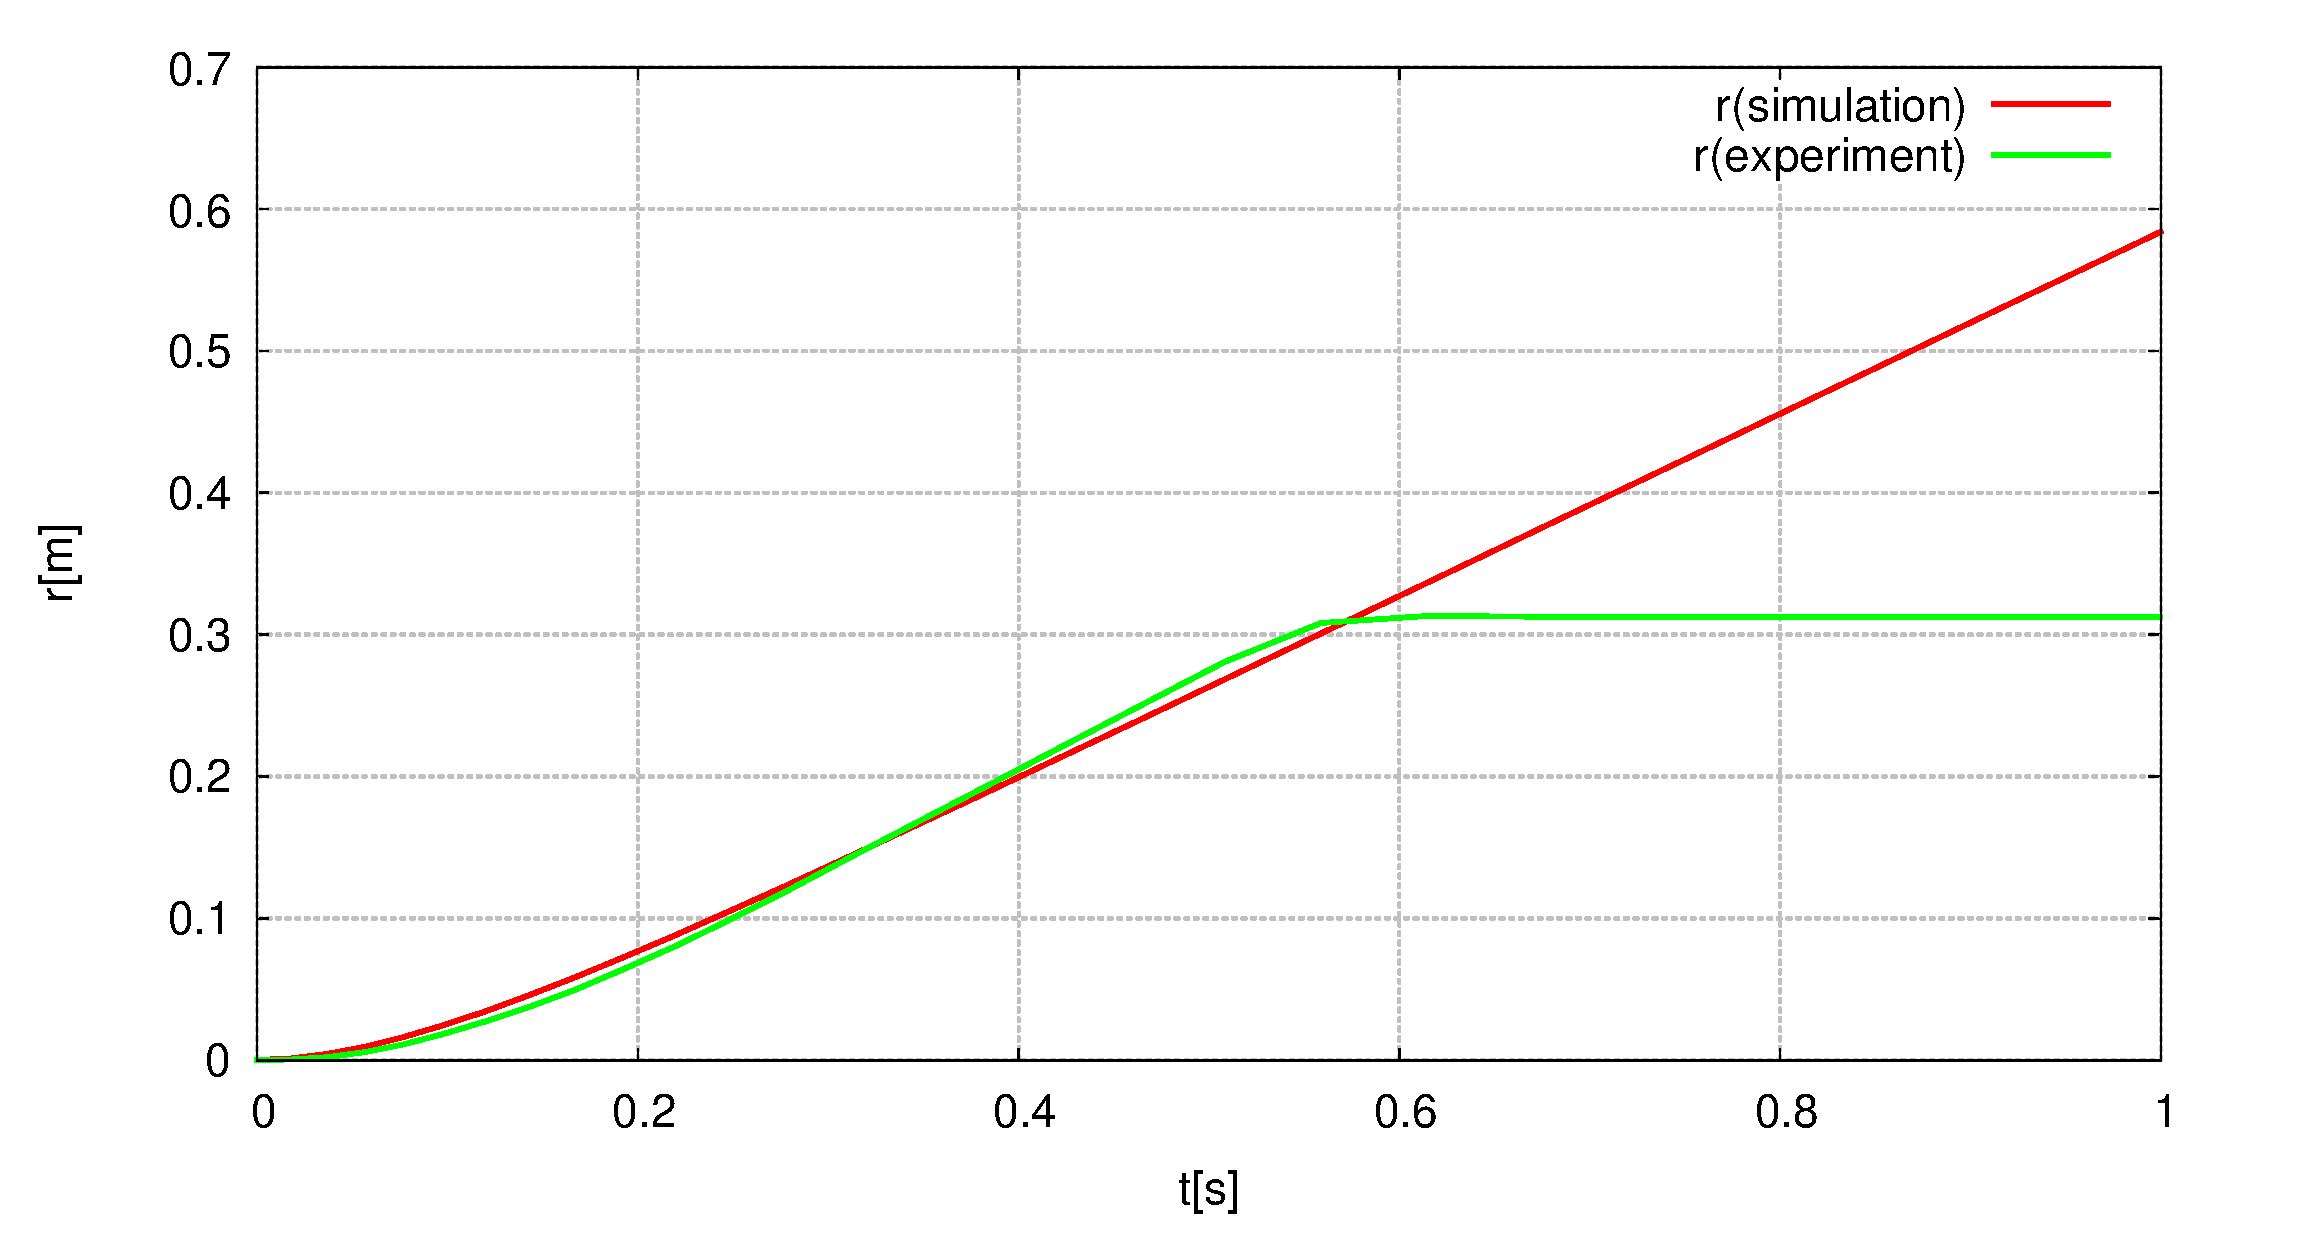
\includegraphics[width=0.8\linewidth]{gazo/nabe8.eps}\\
			\caption{台車のステップ応答シミュレーションと実験結果の比較}
			\label{image:step}
		\end{figure}
		図(\ref{image:step})よりシミュレーションと実験結果に少し差異はあるが
		大きな違いはないといえる。0.6秒以降のグラフが大幅に異なっているが、これはシミュレーションの場合は
		台車の可動範囲に制限がないためずっと台車が移動し続けるが、実験の場合は台車の可動範囲に
		制限があるため、ある時間を境に移動が止まっている。また、このときの入力電圧は$8[\rm{V}]$
		である。以上から同定したパラメータ$M,f,a$は有効な値といえる。
		\newpage
	\subsection{台車のフィードバック応答シミュレーション}
		ここでは、$M,f,a$の検証を行う。$M,f$はフィードバックによる方法で求めた値を用いる。
		%ここの画像はあやしいので差し替え推奨
		以下にシミュレーションと実験データを描画したグラフを示す。ただし、フィードバックゲインは$1500$である。
		\begin{figure}[H]
			\centering
			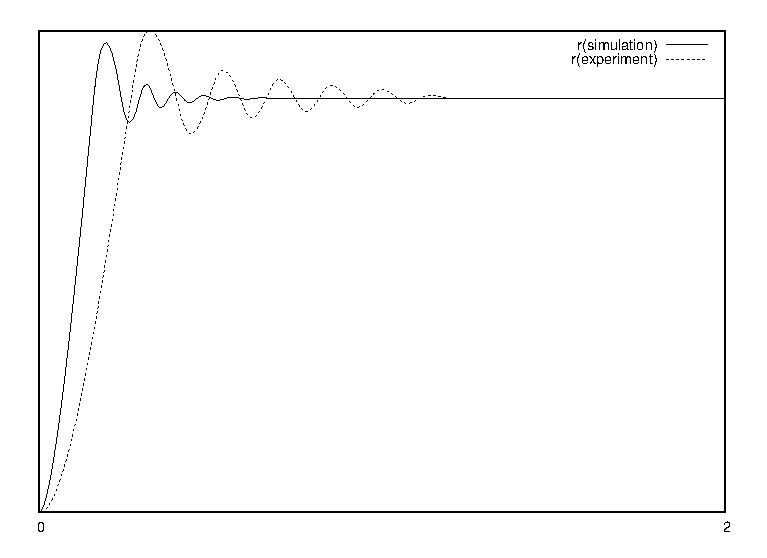
\includegraphics[width=0.8\linewidth]{gazo/feedbackExperiment.eps}
			\caption{フィードバックによる方法のシミュレーションと実験結果の比較}
			\label{image:feedback}
		\end{figure}
		図\ref{image:feedback}よりシミュレーションと実験結果には大きな差異があることが確認できる。
		上述した通りこの方法で同定したパラメータは現実の倒立振子系に即しておらず、結果実験で得られた波形との
		比較において大きな違いが出てきてしまう。よってこの方法で同定したパラメータ$M,f$には
		有効性がないといえる。
		
\section{設計(線形)モデルの決定}
	ここまでで、パラメータを同定し、その有効性についても確かめた。よって、同定すべきパラメータを決定できたので
	システム行列A、入力行列B、出力行列Cを\MaTX{}を用いて計算し、倒立振子の線形モデルを確定する。
	\MaTX{}で計算した各行列を以下に示す。
	\begin{equation}
		A=\left[
		\begin{array}{cccc}
			0 & 0 & 1 & 0 \\
			0 & 0 & 0 & 1 \\
			0 & -0.32 & -10.9 & 0.00038 \\
			0 & 50 & 53 & -0.059 \\
		\end{array}
		\right]
	\end{equation}
	\begin{equation}
		B=\left[
		\begin{array}{c}
			0 \\
			0 \\
			0.87 \\
			-4.3 \\
		\end{array}
		\right]
	\end{equation}
	\begin{equation}
		C=\left[
		\begin{array}{cccc}
			1 & 0 & 0 & 0 \\
			0 & 1 & 0 & 0 \\
		\end{array}
		\right]
	\end{equation}
	ただし、倒立振子を立たせることを目的とするので、上向きを基準としたときの線形状態方程式である。
	%一次チェック完了:
	%---------------------------------------------------------------